  \documentclass{mynotes}

%\geometry{showframe}% for debugging purposes -- displays the margins

\newcommand{\E}{\mbox{E}}
\newcommand{\prox}{ \mathop{\mathrm{prox}} }
\newcommand{\enorm}[1]{\Vert #1 \Vert_2}



\usepackage{amsmath}
%\usepackage[garamond]{mathdesign}

% Set up the images/graphics package
\usepackage{graphicx}
\setkeys{Gin}{width=\linewidth,totalheight=\textheight,keepaspectratio}
\graphicspath{{graphics/}}

\title[Exercises 6 $\cdot$ SDS 385]{Exercises 6: The proximal gradient method}
%\author[ ]{ }
\date{}  % if the \date{} command is left out, the current date will be used

% The following package makes prettier tables.  We're all about the bling!
\usepackage{booktabs}


  \hypersetup{%
    colorlinks=TRUE
  }

% The units package provides nice, non-stacked fractions and better spacing
% for units.
\usepackage{units}

% The fancyvrb package lets us customize the formatting of verbatim
% environments.  We use a slightly smaller font.
\usepackage{fancyvrb}
\fvset{fontsize=\normalsize}

% Small sections of multiple columns
\usepackage{multicol}

% Provides paragraphs of dummy text
\usepackage{lipsum}

% These commands are used to pretty-print LaTeX commands
\newcommand{\doccmd}[1]{\texttt{\textbackslash#1}}% command name -- adds backslash automatically
\newcommand{\docopt}[1]{\ensuremath{\langle}\textrm{\textit{#1}}\ensuremath{\rangle}}% optional command argument
\newcommand{\docarg}[1]{\textrm{\textit{#1}}}% (required) command argument
\newenvironment{docspec}{\begin{quote}\noindent}{\end{quote}}% command specification environment
\newcommand{\docenv}[1]{\textsf{#1}}% environment name
\newcommand{\docpkg}[1]{\texttt{#1}}% package name
\newcommand{\doccls}[1]{\texttt{#1}}% document class name
\newcommand{\docclsopt}[1]{\texttt{#1}}% document class option name

\newcommand{\N}{\mbox{N}}
\newcommand{\thetahat}{\hat{\theta}}
\newcommand{\sigmahat}{\hat{\sigma}}
\newcommand{\betahat}{\hat{\beta}}


\begin{document}

\maketitle% this prints the handout title, author, and date

\bigskip

In this set of exercises, we learn about the proximal gradient algorithm.  This is our first all-purpose algorithm capable of handling non-smooth terms that enforce sparsity, like an $\ell^1$ regularizer.

\section{Proximal operators}

First, some definitions.  Let $f(x)$ be a convex function.  The \textit{Moreau envelope} $E_{\gamma} f(x)$ and \textit{proximal operator} $\prox_{\gamma} f(x)$ for parameter $\gamma > 0$ are defined as
\begin{eqnarray}
E_{\gamma} f(x) &=& \min_{z } \left\{f(z) + \frac{1}{2\gamma} \enorm{z - x}^2  \right\}  \leq f(x) \\
\prox_{\gamma} f(x) &=& \arg \min_{z } \left\{  f(z)+ \frac{1}{2\gamma} \enorm{z - x}^2  \right\} \, .
\end{eqnarray}
Intuitively, the Moreau envelope is a regularized version of $f$.  It approximates $f$ from below, and has the same set of minimizing values as $f$.  The proximal mapping returns the value that solves the little minimization problem defined by the Moreau envelope.  The objective in this little minimization problem balances two goals: minimizing $f$, and staying near $x$.  The proximal operator says \textit{where} the minimum occurs, while the Moreau envelope says what the \textit{value} of the minimum is.

The following figure shows a simple one-dimensional example of a Moreau envelope and a proximal operator for the absolute-value function.

\begin{figure}
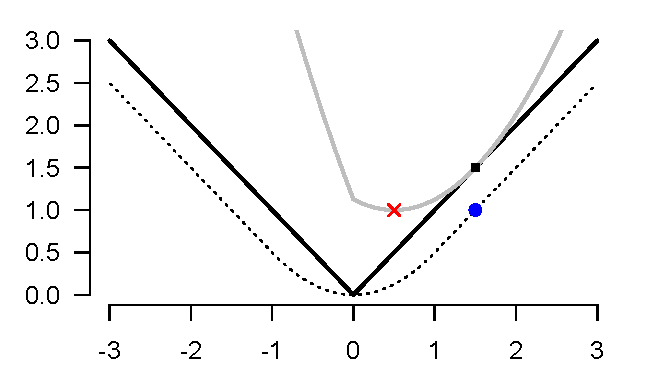
\includegraphics{moreau_envelope.pdf}
\caption{This picture shows a simple example of a proximal operator and Moreau envelope.  The solid black line shows the function $f(x) = |x|$, and the dotted line shows the corresponding Moreau envelope $E_{\gamma} f (x)$ with parameter $\gamma=1$.  The grey line shows the function 
  $|x| + (1/2)(x-x_0)^2$ for $x_0 = 1.5$, whose minimum (shown as a red cross)
  defines the Moreau envelope and proximal operator.  This point has horizontal coordinate
  $\prox_\gamma f(x_0) = 0.5$ and vertical coordinate $E_{\gamma} f (x) = 1$, and is closer than $x_0$
  to the overall minimum at $x=0$.  The blue circle shows the point 
  $(x_0, E_{\gamma} f (x_0))$; the vertical coordinate of the blue point is precisely the vertical coordinate of the red point, emphasizing the point-wise construction of the Moreau
  envelope in terms of a simple optimization problem.
}
\end{figure}

\begin{enumerate}[(A)]
\item
The proximal operator gives a nice interpretation of classical gradient descent.  Consider the local linear approximation of $f(x)$ about a point $x_0$:
$$
f(x) \approx \hat{f}(x; x_0) = f(x_0) + (x - x_0)^{(t)} \nabla f(x_0) \, .
$$

Derive the proximal operator (with parameter $\gamma$) of the linear approximation $\hat{f}(x; x_0)$, and show that this proximal operator is identical to a gradient-descent step for $f(x)$ of size $\gamma$, starting from the point $x_0$.  In reflecting on this answer, make sure you feel comfortable with the following statement: ``the gradient step minimizes a local linear approximation of the function, subject to a quadratic regularizer that keeps the next iterate close to $x_0$ (where, presumably, the linear approximation is reasonable).''

\item Many intermediate steps in statistical optimization problems can be written very compactly in terms of proximal operators of log-likelihoods or penalty functions.  For example, consider a negative log likelihood of the form
$$
l(x) = \frac{1}{2} x^{T} P x - q^{T} x + r \, .
$$
Show that the proximal operator with parameter $1/\gamma$ of $l(x)$ takes the form
$$
\prox_{1/\gamma} l(x) = (P + \gamma I)^{-1} (\gamma  x + q) \, ,
$$
assuming the relevant inverse exists. 

Then show that if we have a Gaussian sampling model of the form $(y \mid x) \sim \N(Ax, \Omega^{-1})$, then our negative log likelihood can be written in the form given above.  Here $A$ is like our feature matrix, $\Omega$ is a covariance matrix, and $x$ is like a regression vector.\footnote{This is notation from the optimization literature, rather than the stats literature.  It's important to be able to translate between both.}  Specify what $P$, $q$, and $r$ are for this negative log likelihood.

\item  Let $\phi(x) = \tau \Vert x \Vert_1$.  Express the proximal operator of this function in terms of the soft-thresholding function that we learned about in the last set of exercises.  (An element-wise expression is fine.)

\end{enumerate}


\section{The proximal gradient method}

Suppose that we have some objective function that can be expressed as $f(x) = l(x) + \phi(x)$, where $l(x)$ is differentiable but $\phi(x)$ is not.  The proximal gradient method is designed for precisely this situation.

Recall from above the idea of forming a local linear approximation to a function at some point $x_0$ and then adding a quadratic regularizer.  This gave us an interpretation of gradient descent evaluating the proximal operator of our locally linear approximation.

Here, we'll apply this idea to the first term in our objective, $l(x)$. Define
$$
l(x) \approx \tilde{l}(x; x_0) = l(x_0) + (x - x_0)^{(t)} \nabla l(x_0) + \frac{1}{2\gamma} \enorm{x - x_0}^2 \, 
$$
as our linear approximation to $l(x)$, plus the quadratic regularizer.  Now we add in the $\phi(x)$ term to get the approximation for our original objective:
\begin{equation}
\label{eqn:pg_approx}
f(x) \approx \tilde{f}(x; x_0) = \tilde{l}(x; x_0) + \phi(x)   \, .
\end{equation}

\begin{enumerate}[(A)]
\item Consider the surrogate optimization problem in which we minimize the approximation $\tilde{f}(x; x_0)$ in Equation \ref{eqn:pg_approx}, in lieu of our original objective $f(x)$. 
$$
\hat{x} = \arg \min_x \; \left\{   \tilde{l}(x; x_0) + \phi(x)  \right\} \, .
$$
Show that the solution to this problem is of the form
\begin{equation}
\label{eqn:pg_xhat}
\hat{x} = \prox_{\gamma} \phi(u) \, , \quad \mbox{where} \quad u = x_0 - \gamma \nabla l(x_0) \, .
\end{equation}
This is just the proximal operator of the non-smooth part of the objective, $\phi(x)$, evaluated at an intermediate gradient-descent step for the smooth part, $l(x)$.


\item The \textit{proximal gradient} method is an iterative algorithm in which we repeatedly form the approximation in Equation \ref{eqn:pg_approx} about the current point, and minimize this surrogate function using Equation \ref{eqn:pg_xhat}.  Written concisely,
$$
x^{(t+1)} = \prox_{\gamma^{(t)}} \phi(u^{(t)}) \, , \quad u^{(t)} = x^{(t)} - \gamma^{(t)} \nabla l(x^{(t)}) \, .
$$

Now consider the lasso regression problem:
$$
\hat{\beta} = \arg \min_{\beta} \left\{  \enorm{y - X\beta}^2 + \lambda \Vert \beta \Vert_1 \right\} \, .
$$
Using the results on proximal operators you've derived already, write down some concise pseudo-code for using the proximal gradient algorithm to minimize this objective.  Identify the primary computational costs of this algorithm.

Now implemement the method and apply it to the diabetes data from last week.  Make sure you track the convergence of the algorithm, i.e.~the objective values over time.  Compare your answers to the answers you get from the package software you used last week (i.e.~\verb|glmnet| or scikit-learn).\footnote{Keep in mind that those packages are using a value of $\lambda$ that is rescaled by a factor of $n$, since they use the loss function
$$
\frac{1}{2n} \enorm{y - X\beta}^2  + \lambda \Vert \beta \Vert_1 \, .
$$
}

\item A cool variation on proximal gradient is called the \textit{accelerated} proximal gradient algorithm.   The following scheme (due to Nesterov, who's super famous in this area) involves a simple extrapolation step based on the previous iteration:
$$
\begin{aligned}
x^{(t+1)} &= \prox_{ \gamma^{(t)}} \phi(u^{(t)}) \, , \quad u^{(t)} =  z^{(t)} - \gamma^{(t)} \nabla l(z^{(t)})  \\
s^{(t+1)} &= \frac{1 + (1 + 4 s_{t}^2)^{1/2}}{2} \\
z^{(t+1)} &=  x^{(t+1)} + \left( \frac{s^{(t)} - 1}{s^{(t+1)}} \right) (x^{(t+1)} - x^{(t)}) \, .
\end{aligned}
$$



The first step involves the proximal operator of the penalty function, evaluated not at the previous iterate $x^{(t)}$, but at an extrapolated version of $x^{(t)}$, based on the magnitude of the previous step's update.  In this sense, large steps give ``momentum'' to the next step, where the amount of momentum is modulated by the scalar $s^{(t)}$ terms.

Implement this acceleration scheme in your proximal gradient code, and compare its convergence speed to that of the unacceleration version.  Does the value of the objective goes down at each and every step?  Do you get to the minimum faster?

Note: you can use this acceleration trick in ordinary gradient descent, too.

\end{enumerate}


\end{document}




